
\documentclass[10pt]{article}
\usepackage[margin=1in]{geometry}
\usepackage{amsmath}
\usepackage{amssymb}
\usepackage{setspace}
\usepackage{graphicx}
\usepackage{caption}
\usepackage{listings}
\usepackage{enumitem}
\usepackage{subfigure}


\begin{document}

\title{ECE 4750 Lab 5: Multicore Processor}
\author{Avinash Navada (abn44) \& Akshay Dongaonkar (akd54) 
		\& Vivek Gaddam (vrg22)}
\maketitle


\section{Introduction}

Modern computing applications are increasingly calculation-intensive, highlighting the 
need for systems capable of parallelizing work over multiple execution cores to keep 
total program execution time reasonably low. However, such systems come with
added complexity, and their success relies on design choices, such as the particular
cache and on-chip interconnect network schemes to use. \par

In this lab, we seek to analyze the benefits of using a quad-core system with
a banked data cache and private instruction caches over a single-core system with a data
and instruction cache by comparing their performance on a set of serial and parallel microbenchmarks.
In doing so, we can gain insight into the specific area, energy, and performance tradeoffs between these setups
and draw conclusions on when one system might be more appropriate than the other.

The baseline design is the single-core setup, and the alternative design is the quad-core setup.
In completing both designs, we ultimately found that the alternative design performed better on ...
% INSERT QUANTITATIVE RESULTS HERE!!!! in terms of the number of cycles executed
% INSERT EFFECT OF ALT ON AREA, ENERGY, CYCLE TIME
Based on these results, we can say that we generally expect ...



\section{Project Management}

% 
For this lab, all testing was provided. Therefore, we split the remainder of the work amongst ourselves as follows:
-Avinash wrote the RTL code for the baseline and alternative designs composing the processor cores, caches, and network
-Akshay wrote the version of the quicksort algorithm to be run on the baseline design and parallelized it for testing on the alternative design
-Vivek helped optimize the quicksort C algorithm and was the lead in writing the lab report


\section{Baseline Design}

The baseline design for this lab report is a single-core system consisting of a bypassed pipelined PARCv2 
processor, a two-way set-associative instruction cache, and a two-way set-associative data cache. 

Due to an existing bug in our pipelined processor from Lab 2, we decided to use the provided processor core, 
cache, and network units in composing our baseline design. Our design is in accordance with the setup in 
Figure~\ref{fig:bline}. This overall setup is responsible for taking assembly instructions from a provided
instruction memory and interfacing with a provided data memory in order to execute programs.

Because our baseline design is composed entirely of components that were designed in previous labs that were 
tested individually, specifically the caches and processor core, it is a good example of a modular design. 

This design can be viewed as the minimum hardware one expects to have when running full C programs, and is therefore
an appropriate baseline for comparison for more complicated designs, such as the quad-core processor that serves as
our alternative design. Any real system includes caches for instruction and data memories to reduce the average memory
access latency (AMAL), so it makes sense for our baseline implementation to use them as well. 

As part of the requirements of completing the baseline design, we implemented the quicksort algorithm in C for use on
one core. This was used as a microbenchmark in our lab. The provided quicksort method signature contains a A slight optimization that we provided in our lab was to amortize
because this eliminates , this should 

% Diagram of base datapath or block diagram


\section{Alternative Design}

In our alternative design, which is a quad-core system, we use four processor cores like the one in the baselign design and compose them with four two-way set-associative instruction caches, one per core, and one two-way set-associative data cache unit.An interconnect network supports communication between the cores. See Figure~\ref{fig:alt} for the datapath of our alternative design.

We would like to see how close our alternative design can come to actually realizing the ideal performance benefit of having four cores with the knowledge that the additional network infrastructure required to make such a design work comes with some energy and performance cost.


\section{Testing Strategy}

As mentioned earlier, the testing code for this lab was provided. The general testing approach taken here was to have a test for each microbenchmark ...



\section{Evaluation}

% 


\newpage
\section {Tables and Diagrams}

% Figure: Gantt Chart
% \begin{figure}[h]
% 	\centering
% 	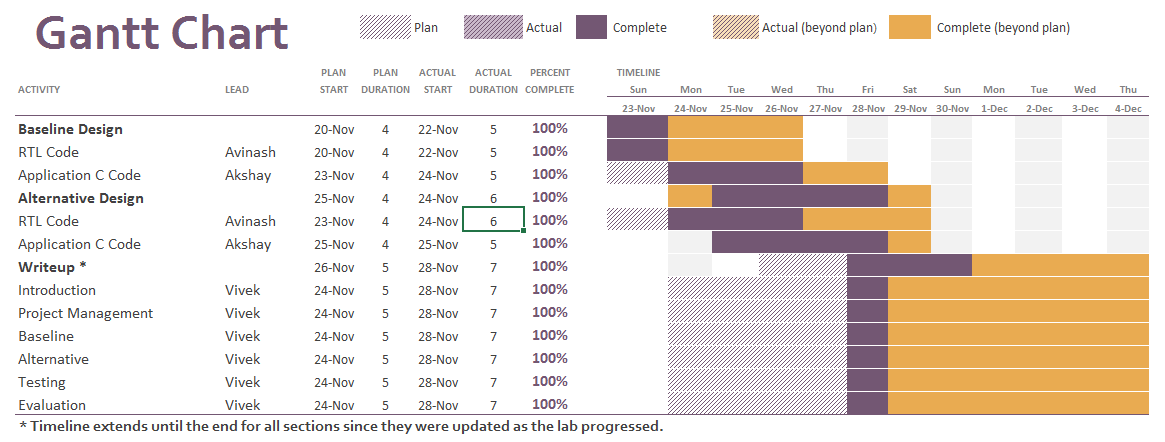
\includegraphics[scale=0.4, angle=90]{gantt}
% 	\caption{Gantt Chart.}
% 	\label{fig:gantt}
% \end{figure}

% Figure: Baseline datapath
\begin{figure}[h]
	\centering
	\label{fig:bline}
	\caption{????}
\end{figure}



\end{document}






